\section{Improved CSC Trigger Algorithm for High Luminosity Running}
\label{sec:SLHC_algo}

\subsection{Separate finding of CLCTs in ME1/a and ME/1b}

 In the old TMB f/w, the 16 ganged strip channels from ME1/a are appended to the 64 ME/1b strip channels and the reconstruction of CLCTs is performend as if it's a single regular chamber with 80 channels (is there any treatment of the boundary, so that ME1/a strips are not combined with ME1/b strips?). The two rather separate and distinctive areas combined and treated like one uniform unit with the maximum of two CLCT stubs on the output.

With unganged ME1/a and higher pile-up such a simple approach becomes increaingly unnatural and ineffective. The ME1/a would have x3 more channels now, so it would deserve to be treated like a seperate chamber even more. And chances to get multiple stubs are increasing with higher luminosity, especially so in ME1/a. With multiple stubs, the stubs in ME1/a would start directly competing with those in ME1/b.

With a larger size FPGA, it would be beneficial to treat ME1/a and ME1/b as two separate chambers for the purpose of CLCT reconstruction, with each area having their own limit on the maximum of 2 CLCTs. Thus, the whole ME1/1 would be able to have maximum 4 CLCTs available for matching with ALCTs. It's important to keep more 2D stubs available so that at the stage of matching we can reduce the number of stubs following some better tuned criteria.

Finally, in the case if we would allow to read out the 2D CLCT stubs without an ALCT match, and we cannot read out more then 2 of them per BX per ME1/1, we can device a selection criteria when comparing stubs from ME1/a and 1/b as follows: e.g., if quality of an ME1b stub is the same or less by one then that of an MEr 1a stub, prefer the ME1b one. 

\subsection{Localizing the TMB dead time }

 The main source of the old TMB inefficiency in high pile-up is the dead time which happens for the whole ME1/1 chamber after there was a triggering CLCT. The TMB's state-machine freezes whole TMB for several BXs after a CLCT trigger while number of coincidence layers stays over the trigger threshold. If anywhere in a chamber there was an CLCT from PU a few BX earlier before a signal muon, it would be impossible to trigger on the signal.

While it's clear that with the comparator information which we recieve in TMB, it's not really possible to distinguish close in time signals in the same strip, there seem to be no apparent reason, other then the complexity of the algorithm, for this dead time to be present in strips that had no trigger.

Thus, the algorithm approach to deal with this issue for the upgrade could be as follows:
\begin{itemize}
    \item when a CLCT trigger happens, mark as busy only those strips within either a fixed dead time zone around CLCT (8 half-strips, see "useDeadTimeZoning" parameter in Sec.~\ref{sec:CLCT_conf}) or within the dead time zone, the width of which depends on the CLCT pattern (from 11 half-strips for the most bent patterns to 3 half-strips for the straightest one, see "useDynamicStateMachineZone" parameter in Sec.~\ref{sec:CLCT_conf}), and also mark the signal half-strip that specifies the triggered CLCT
    \item during the following bunch-crossings, check if the number of coincidence layers drops under the trigger threshold for the signal half-strip
    \begin{itemize}
	\item if it does, remove the "busy" mark from the corresponding strips 
    \end{itemize}
    \item if strips are marked as busy in a BX, they are excluded from pattern recognition 
\end{itemize}

\subsection{Restriction of CLCT pattern bend }

 The current set of CLCT patterns (e.g., see p5 of TMB2005\_spec\_v4p55) is largely geared towards low pt tracks. For tracks with pt>10, only the straighest and the next one bent patterns are significant. The restriction on allowed pattern bending would significantly help with many issues including multiplicity \& rate, ghosting, dead-time and corresponding loss of the efficiency (see "clctPidThreshPretrig" parameter in Sec.~\ref{sec:CLCT_conf}). Positive effect of it would increase with increasing luminosity. However, it would also somewhat reduce the efficiency because of not so good pt-threshold resolution from fairly narrow (11cm) CSC chambers, especially for medium to lower pt muons.

TODO: need a plot showing the efficiency vs pt for a simtrack to have a matching reconstricted CLCT stub for different maximum thresholds for the bend. GEMs could be helpful for improving the effectivenes and the efficiency of the bend restriction. 

\subsection{Improving CLCT timing }

 Currently, the BX time of a CLCT stub is defined as the BX of its pretrigger. Or, in other words, it's first BX when at least three layers fit one of the CLCT patterns. Note that an attempt to latch a trigger pattern is performed after the number of BX after the pretrigger defined by the clctDriftDelay parameter (=2BX). And also note that a CLCT pattern during the pretrigger could be different then the one that happen to match during the trigger.

With higher luminosity there are increasingly larger chances for some strips in some of the layers to be hit by earlier background hit. And that has chances to affect the time when a pretrigger might be detected. A more robust solution would be to define stub's time using the times of its strips, where stub's strips are defined as strips that were matched within a CLCT pattern during the trigger. As for a specific procedure, a median time over those strips' times or some sort of a truncated average could be used (see "clctUseCorrectedBx" parameter in Sec.~\ref{sec:CLCT_conf}, analogously for "alctUseCorrectedBx" parameter in Sec.~\ref{sec:ALCT_conf}).

\subsection{ALCT Handling }

 It should be possible to improve the efficiency, rate and timing precision of ALCT stubs by, e.g.
\begin{itemize}
    \item tuning of the ghost cancellation logic (ALCTs in neighboring wiregroups, see "alctGhostCancellationBxDepth" and "alctGhostCancellationSideQuality" parameters in Sec.~\ref{sec:ALCT_conf}) and removing pre-trigger deadtime (see "alctPretrigDeadtime" parameter in Sec.~\ref{sec:ALCT_conf});
    \item using more narrow ALCT pattern in ring 1 chambers (see "alctNarrowMaskForR1" parameter in Sec.~\ref{sec:ALCT_conf});
    \item using more precise algorithm (e.g., running median or truncated average) for BX assignment (see "alctUseCorrectedBx"  parameter in Sec.~\ref{sec:ALCT_conf}).
\end{itemize}

However, here we would only like to focus on how the ALCT stubs would be used by TMB.

ALCTs are reconstructed from the signals in layers of anode wires which are ganged into wiregroups and are continuously covering the whole ME1/1 chamber. Most of the wiregroups can only physically cross only strips either in ME1/a or only in ME1/b. A complication specific to ME1/1 is that wires here are not perpendicular to strips, but are slanted at 29 degrees from the straight angle. Thus, some wiregroups are crossing the border between ME1/a and ME1/b. If signal is detercted in such a wiregroup, there is an ambiguity about which part of ME1/1 it might belong to.

For the ALCTs received by TMB we propose to split the incoming stubs into two parts, ME1/a and ME1/b, that would be used further for LCT matching separately in ME1/a and ME1/b. 

\subsection{Narrowing the matching time window }

 The current TMB uses a rather wide time matching window (7BX) that is centered on a CLCT's BX, and is used to look for an ALCT match within it. A wide matching window is not good in high pileup, as propability of incorrect matching with background 2D stubs is higher, resulting in inefficiency.

For the SLHC, we can probably assume that the system is well timed and that we can use the narrowest reasonable matching window of 3BX wide (see "matchTrigWindowSize" parameter in Sec.~\ref{sec:TMB_conf}). 

\subsection{Modification of the stub timing logic in matching }

 In the old TMB algorithm, the stub timing logic works during the 2D stubs matching as follows:
\begin{itemize}
    \item CLCT-centric approach: CLCTs and their BX are taken as reference points, while ALCTs are waiting in a queue
    \item for a BX with CLCTs we look for a first BX in the matching window that has ALCTs
    \item after matching is dome in this BX, the ALCTs from there are taken off the queue, and cannot be matched with any later CLCT (see "tmbDropUsedClcts" and "matchEarliestClctME11Only" parameters in Sec.~\ref{sec:TMB_conf})
\end{itemize}

The main issues with this approach at high luminosity is that when there is an ALCT from a good signal muon, early CLCTs from background might steal it and form wrong match, and this correct ALCT then would not be available anymore for matching with a later correct CLCT.

Proposal to improve the situation:
\begin{itemize}
    \item ALCT-centric approach: ALCTs and their BXs are taken as reference points, while reconstructed CLCTs are waiting in a matching window-wide queue (see "clctToAlct" parameter in Sec.~\ref{sec:TMB_conf})
    \begin{itemize}
        \item ALCT's BX and the middle BX in the matching window-wide queue are expected to be synchronized 
    \end{itemize}
    \item for an ALCT's BX we look for CLCTs within the queue in the order of arrival try to find maximum 2 LCT matches as follows (see "tmbCrossBxAlgorithm" parameter in Sec.~\ref{sec:TMB_conf}):
    \begin{itemize}
        \item first look for CLCTs in the same BX 2) if we didn't get 2 LCT matches yet, look for CLCTs in BX-1
        \item if we didn't get 2 LCT matches yet, look for CLCTs in BX+1
        \item etc... depending on how wide the matching window is 
    \end{itemize}
    \item can optionally either remove CLCTs from the queue after there was an LCT match, or can keep them for reuse possibilities to be matched with later ALCTs (see "tmbDropUsedClcts" parameter in Sec.~\ref{sec:TMB_conf})
    \item NOTE: all this is supposed to be done separately in ME1a and in ME1b 
\end{itemize}

\subsection{Selecting up to two the best LCTs per ME1/1}

With the backplane limitations, we can read out only up to two trigger stubs per BX from the whole ME1/1.

Since ME1/a and ME1/b now can each have up to two stubs, we need an extra step of selecting the best two ME1/1 stubs out of possible 4. If ME1/a + ME1/b has more then two LCTs:
\begin{itemize}
    \item The simplest solution:
    \begin{itemize}
	\item drop the highest eta ones until we have just two. 
    \end{itemize}
    \item Possible improvement:
    \begin{itemize}
        \item rank stubs by special quality value which is the same as stub quality for ME1/b and is stub quality-1 for ME1/a stubs
        \item if special quality is the same, rank by eta 
    \end{itemize}
\end{itemize}

\newpage
\subsection{Sofware Emulation of ALCT Level Improvements}

\subsubsection{Tuning of Ghost Cancellation Procedure}

\textcolor{red}{Current} ghost cancellation:
\begin{itemize}
    \item Loop over wire groups:
    \begin{itemize}
        \item Consider WG = N
        \item Cancel trigger in this wire group if there is trigger in WG = N-1 and:
        \begin{itemize}
            \item with the same BX and with \textcolor{red}{better or equal} quality
            \item up to \textcolor{red}{4} BXs earlier, with \textcolor{red}{any} quality
        \end{itemize}
        \item Cancel trigger in this wire group if there is trigger in WG = N+1 and:
        \begin{itemize}
            \item with the same BX and with \textcolor{red}{better} quality
            \item up to \textcolor{red}{4} BXs earlier, with \textcolor{red}{any} quality
        \end{itemize}
    \end{itemize}
\end{itemize}
\textcolor{blue}{New} ghost cancellation:
\begin{itemize}
    \item Loop over wire groups:
    \begin{itemize}
        \item Consider WG = N
        \item Cancel trigger in this wire group if there is trigger in WG = N-1 and:
        \begin{itemize}
            \item with the same BX and with \textcolor{blue}{better} quality
            \item up to \textcolor{blue}{1} BX earlier, with \textcolor{blue}{better} quality
        \end{itemize}
        \item Cancel trigger in this wire group if there is trigger in WG = N+1 and:
        \begin{itemize}
            \item with the same BX and with \textcolor{blue}{better or equal} quality
            \item up to \textcolor{blue}{1} BX earlier, with \textcolor{blue}{better and equal} quality
        \end{itemize}
    \end{itemize}
\end{itemize}

The following modifications in configuration are related to this improvement:
\begin{itemize}
    \item alctGhostCancellationBxDepth: 4BX to 1BX
    \item alctGhostCancellationSideQuality: False to True
\end{itemize}

\subsubsection{Narrow ALCT Pattern Mask}

Use more narrow ALCT pattern mask for stations in Ring 1 (see Fig.~\ref{fig:narrow_alct_pattern_mask}).

\begin{figure}[tbh]
        \begin{center}
                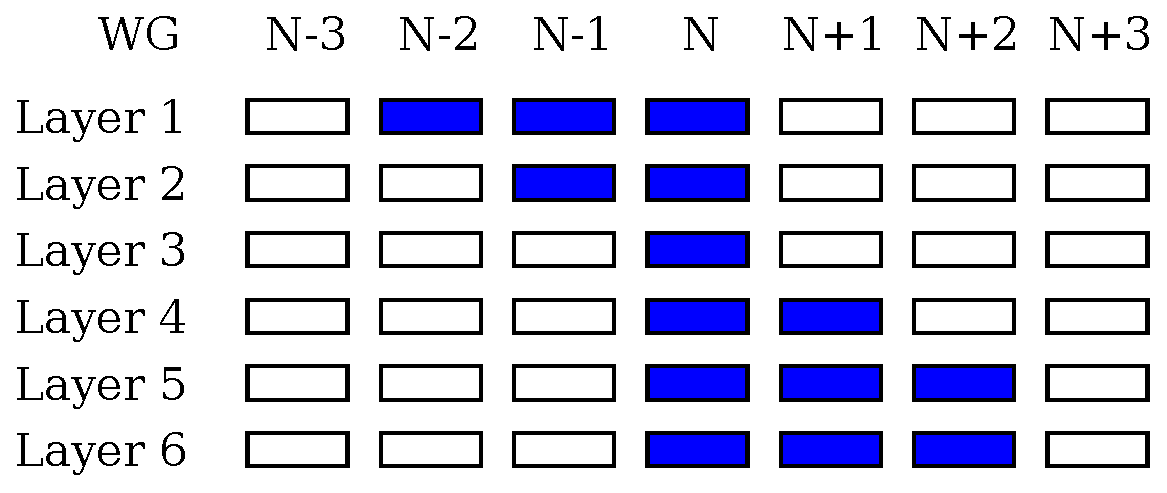
\includegraphics[width=0.49\linewidth]{figures/alct_pretrigger.pdf}\\
                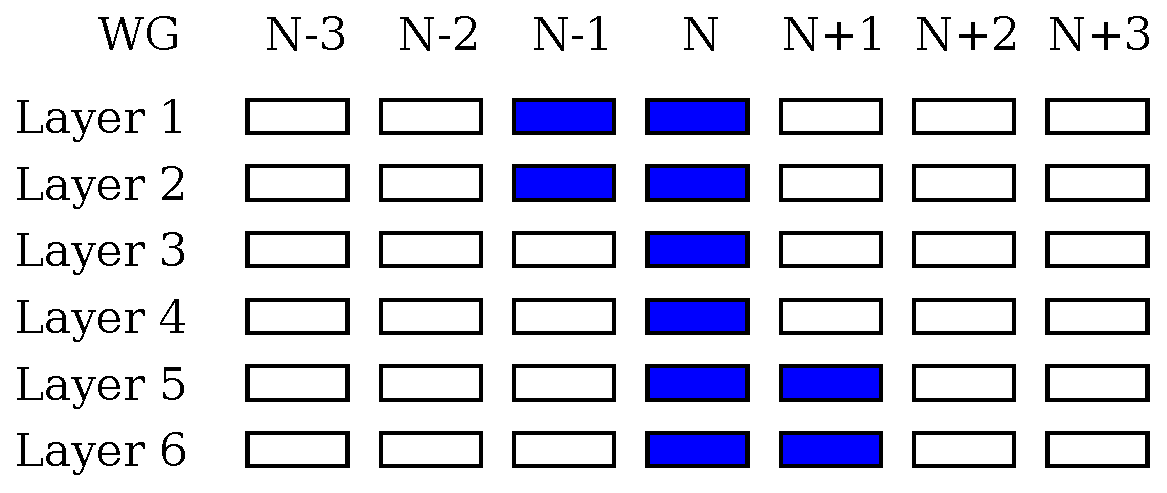
\includegraphics[width=0.49\linewidth]{figures/alct_pretrigger_r1.pdf}
                \caption{Top: default ALCT pattern mask, bottom: narrow ALCT pattern mask.}
                \label{fig:narrow_alct_pattern_mask}
        \end{center}
\end{figure}

The following modifications in configuration are related to this improvement:
\begin{itemize}
    \item alctNarrowMaskForR1: False to True
\end{itemize}

\subsubsection{Reduced ALCT Dead Time}

Currently, if there is pretrigger in BX = B (see Fig.~\ref{fig:alct_deadtime}):
\begin{itemize}
    \item Check for trigger in BX = B + drift time = B+2
    \item Search for next pretrigger starting from BX = B + drift time + extra deadtime = B+6
\end{itemize}

Suggested improvement: decrease extra deadtime from 4 BX to 0 BX.

\begin{figure}[tbh]
        \begin{center}
                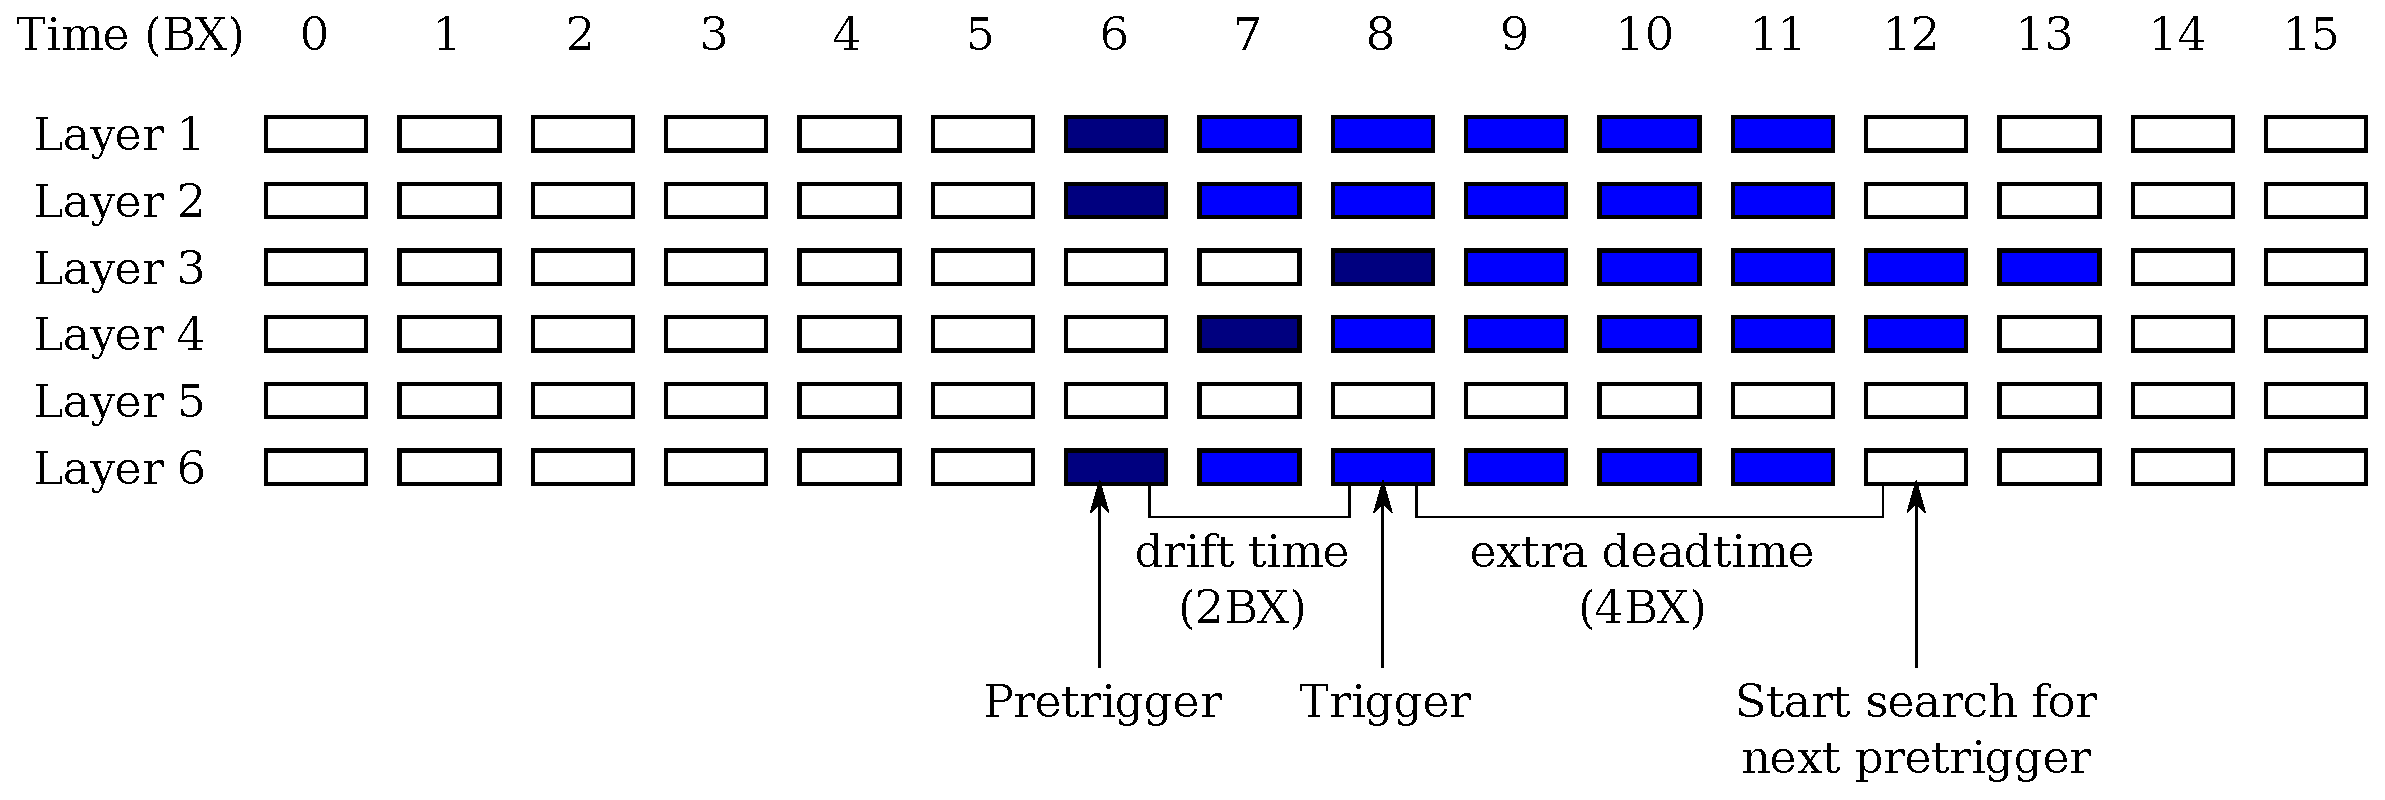
\includegraphics[width=0.98\linewidth]{figures/stretched_hits_alct_deadtime.pdf}
                \caption{Top: Dead Time between ALCT pretriggers.}
                \label{fig:alct_deadtime}
        \end{center}
\end{figure}

The following modifications in configuration are related to this improvement:
\begin{itemize}
    \item alctPretrigDeadtime: 4BX to 0BX
\end{itemize}

\newpage
\subsection{Sofware Emulation of CLCT Level Improvements}

\subsubsection{Localizing Dead Zone}

\textcolor{red}{Current implementation of dead time}:
\begin{itemize}
    \item After constructing up to two CLCTs, \textcolor{red}{continue the loop over all BXs until there is a BX with no triggers}
    \\...
    \item In the BX with trigger, construct up to two CLCTs from two best triggers \textcolor{red}{in all half-strips}
    
\end{itemize}
\textcolor{blue}{New implementation of dead time}:
\begin{itemize}
    \item After constructing up to two CLCTs, \textcolor{blue}{mark 16 half-strips around half-strips of these CLCTs as busy while number of hit layers in half-strips of these CLCTs $\geq$ 4}
    \item \textcolor{blue}{After trigger in BX = B, keep searching for pretrigger in strating from BX = B+1}
    \\...
    \item In the BX with trigger, construct up to two CLCTs from two best triggers \textcolor{blue}{in half-strips}
    \begin{itemize}
        \item \textcolor{blue}{within 5 half-strips from pretrigger half-strips}
        \item \textcolor{blue}{which are not marked as busy from previous trigger}
    \end{itemize}
\end{itemize}

The following modifications in configuration are related to this improvement:
\begin{itemize}
    \item useDeadTimeZoning: False to True
\end{itemize}

\subsubsection{Dynamic Dead Zone Width}

\textcolor{red}{Fixed dead time zone}:
\begin{itemize}
    \item After constructing up to two CLCTs, mark \textcolor{red}{16} half-strips around half-strips of these CLCTs as busy while number of hit layers in half-strips of these CLCTs $\geq$ 4
\end{itemize}
\textcolor{blue}{Dynamic dead time zone}:
\begin{itemize}
    \item After constructing up to two CLCTs, mark \textcolor{blue}{K(pid)} half-strips around half-strips of these CLCTs as busy while number of hit layers in half-strips of these CLCTs $\geq$ 4
\end{itemize}
\vskip3mm
K(pid) --- function of pattern id:
\begin{itemize}
    \item K(1,2,3) = 22 half-strips
    \item K(4,5) = 18 half-strips
    \item K(6,7) = 14 half-strips
    \item K(8,9) = 10 half-strips
    \item K(10) = 6 halt-strips
\end{itemize}

The following modifications in configuration are related to this improvement:
\begin{itemize}
    \item useDynamicStateMachineZone: False to True
\end{itemize}

\newpage

\subsubsection{Minimal Pattern ID for Pretriggering}

\textcolor{red}{Current CLCT pretrigger}:
\begin{itemize}
    \item Loop over all BXs (starting from BX = 0) and all half-strips:
    \begin{itemize}
        \item Count number of layers with hits in the following patterns
        \item If this number $\geq$ 3: pretrigger occurs
        \item Accept this pretrigger if its pattern id $\geq$ \textcolor{red}{2}
    \end{itemize}
\end{itemize}
\textcolor{blue}{New CLCT pretrigger}:
\begin{itemize}
    \item Loop over all BXs (starting from BX = 0) and all half-strips:
    \begin{itemize}
        \item Count number of layers with hits in the following patterns
        \item If this number $\geq$ 3: pretrigger occurs
        \item Accept this pretrigger if its pattern id $\geq$ \textcolor{blue}{4}
    \end{itemize}
\end{itemize}

The following modifications in configuration are related to this improvement:
\begin{itemize}
    \item clctPidThreshPretrig: 2 to 4
\end{itemize}

\subsubsection{Minimal Separation Between Two Best CLCTs}

\textcolor{red}{Current construction of up to two CLCTs}:
\begin{itemize}
    \item Search for the best trigger in this BX
    \item Mark \textcolor{red}{20} half-strips around the best trigger as busy
    \item Find the second best trigger among non-busy half-strips
\end{itemize}
\textcolor{blue}{New construction of up to two CLCTs}:
\begin{itemize}
    \item Search for the best trigger in this BX
    \item Mark \textcolor{blue}{10} half-strips around the best trigger as busy
    \item Find the second best trigger among non-busy half-strips
\end{itemize}

The following modifications in configuration are related to this improvement:
\begin{itemize}
    \item clctMinSeparation: 10 to 5 cathode strips
\end{itemize}

\newpage
\subsection{Sofware Emulation of TMB Level Improvements}

\subsubsection{Decreased Trigger Matching Window}

Decrease size of trigger matching time window from 7 BXs to 3 BXs (see Fig.~\ref{fig:clct_alcts_short_window}).

\begin{figure}[tbh]
        \begin{center}
                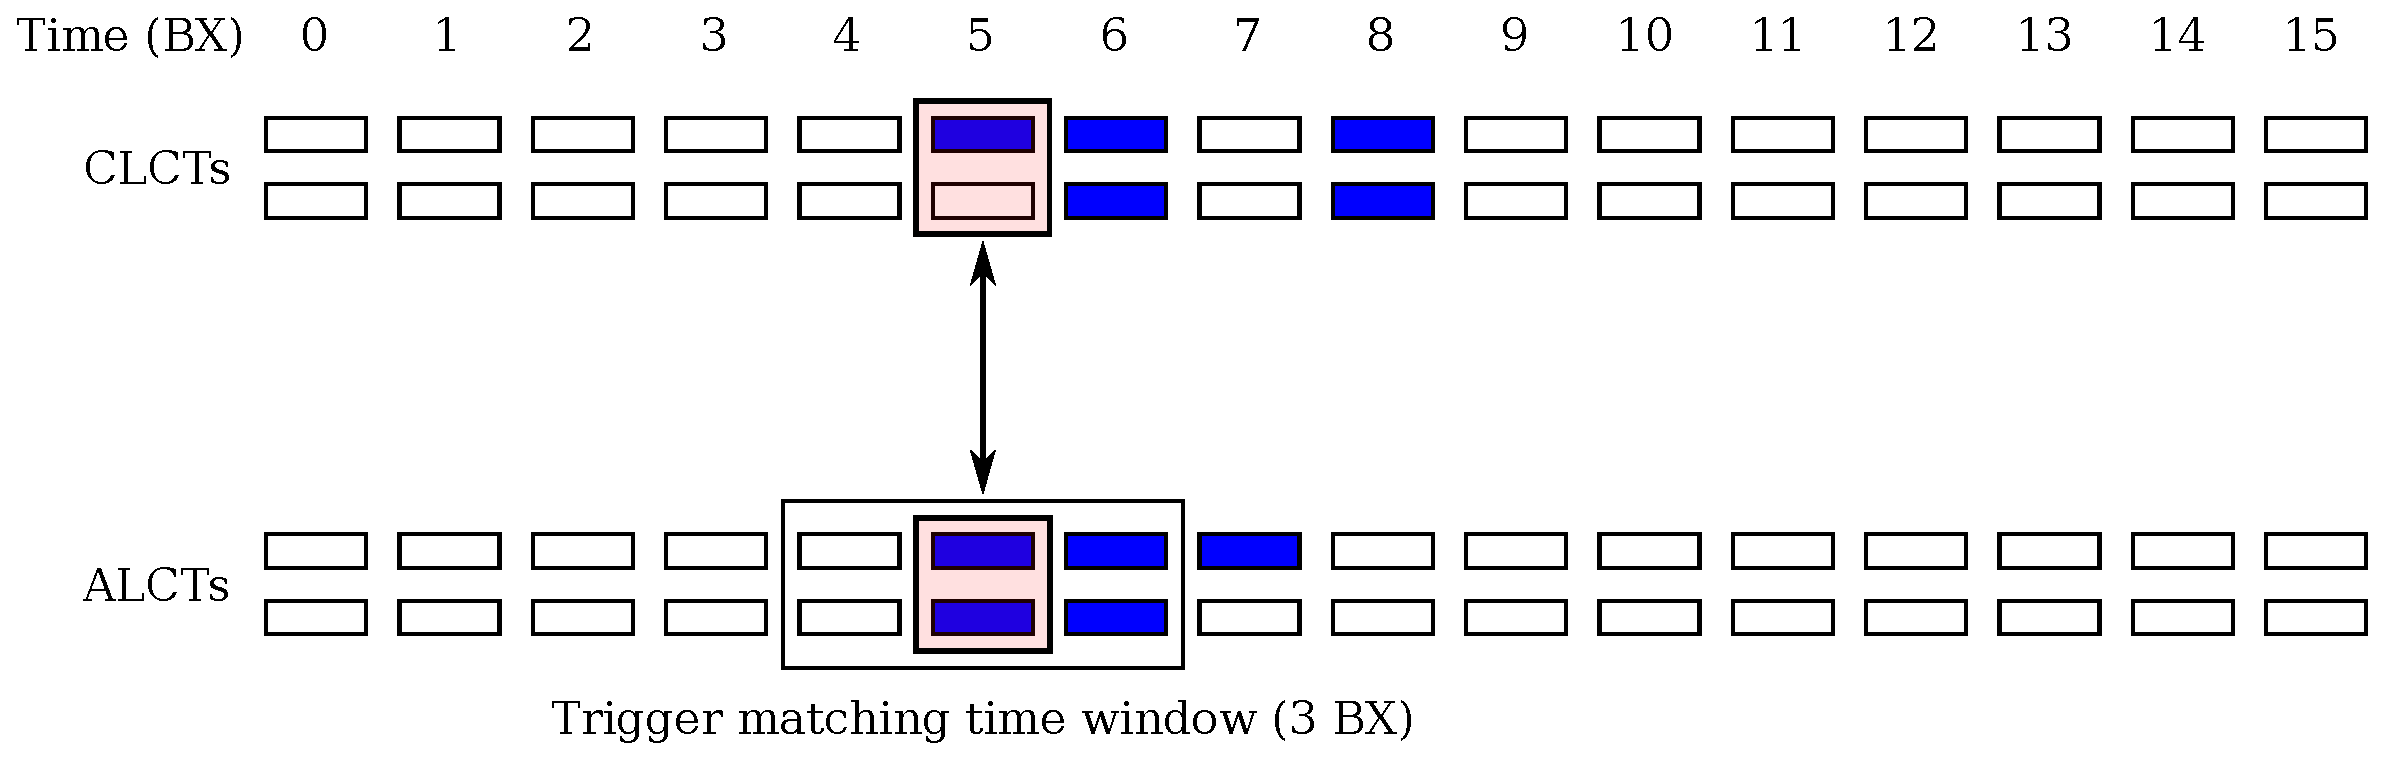
\includegraphics[width=0.98\linewidth]{figures/clct_alcts_short_window.pdf}
                \caption{Decreased trigger matching window.}
                \label{fig:clct_alcts_short_window}
        \end{center}
\end{figure}

The following modifications in configuration are related to this improvement:
\begin{itemize}
    \item matchTrigWindowSize: 7BX to 3BX
\end{itemize}

\subsubsection{ALCT-centric ALCT and CLCT Correlation}

Switch from CLCT-centric matching to ALCT-centric matching (see Fig.~\ref{fig:alct_clcts}).

\textcolor{red}{CLCT-centric matching}
\begin{itemize}
    \item Loop over CLCT BXs from BX = 0 to BX = 15
    \item For CLCT BX = B with at least one valid CLCT:
    \begin{itemize}
        \item Loop over ALCT BXs from BX = B-3 to BX = B+3
    \end{itemize}
\end{itemize}
\textcolor{blue}{ALCT-centric matching}
\begin{itemize}
    \item Loop over ALCT BXs from BX = 0 to BX = 15
    \item For ALCT BX = B with at least one valid ALCT:
    \begin{itemize}
        \item Loop over CLCT BXs from BX = B-3 to BX = B+3
    \end{itemize}
\end{itemize}

\begin{figure}[tbh]
        \begin{center}
                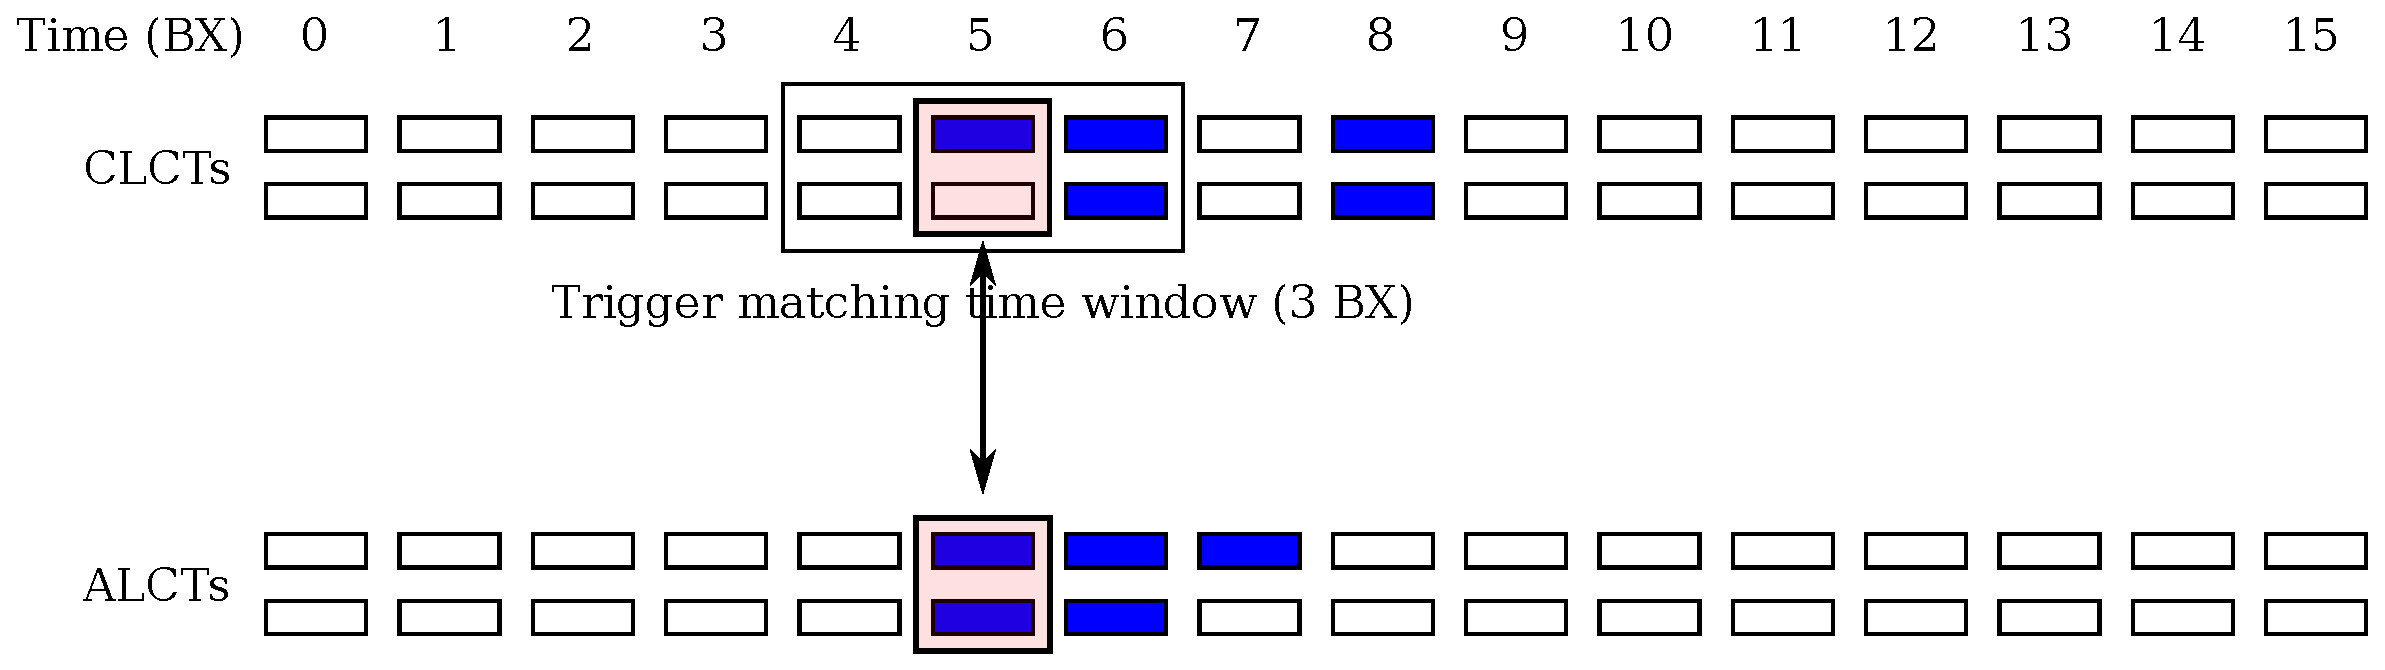
\includegraphics[width=0.98\linewidth]{figures/alct_clcts.pdf}
                \caption{ALCT-centric ALCT anc CLCT correlation.}
                \label{fig:alct_clcts}
        \end{center}
\end{figure}

The following modifications in configuration are related to this improvement:
\begin{itemize}
    \item clctToAlct: True to False
\end{itemize}

\subsubsection{Reusage of Used ALCTs and CLCTs}

Allow reusage of ALCTs and CLCTs already used during ALCT and CLCT correlation (see Fig.~\ref{fig:reuse_alct_clct}).

\textcolor{red}{Current behavior}:
\begin{itemize}
    \item Drop used CLCTs: do not use them with ALCTs in other ALCT BXs;
    \item Proceed to next ALCT BX after matching ALCTs with earliest CLCT BX with at least one valid CLCT.
\end{itemize}
\textcolor{blue}{New behavior}:
\begin{itemize}
    \item Do not drop used CLCTs: reuse them with ALCTs in other ALCT BXs;
    \item Match ALCTs to CLCTs in all CLCT BXs within matching window.
\end{itemize}

\begin{figure}[tbh]
        \begin{center}
                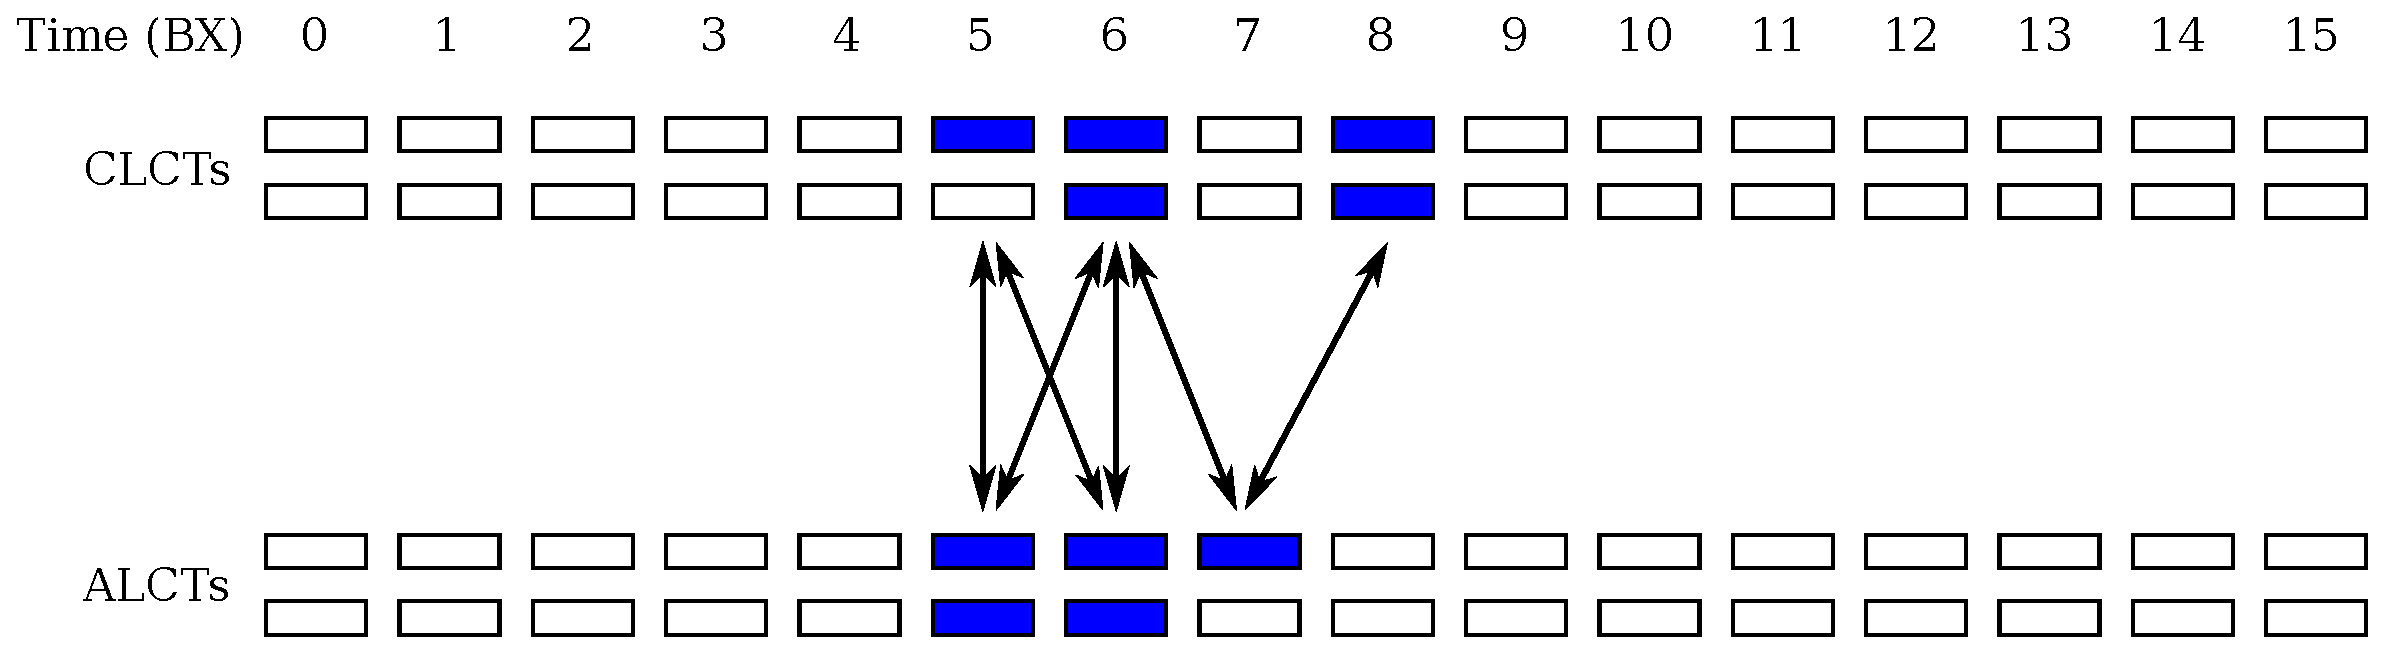
\includegraphics[width=0.98\linewidth]{figures/clct_alcts_end_2.pdf}
                \caption{Reusage of already used ALCTs and CLCTs.}
                \label{fig:reuse_alct_clct}
        \end{center}
\end{figure}

The following modifications in configuration are related to this improvement:
\begin{itemize}
    \item tmbDropUsedClcts: True to False
    \item matchEarliestClctME11Only: True to False
\end{itemize}

\subsubsection{Cross BX Algorithm}

In the situation shown on Fig.~\ref{fig:reuse_alct_clct}, in some given BX = B we can end up having with up to 6 LCTs (made from ALCTs in BX = B and CLCTs in BX = B-1, B, B+2. How do we choose two LCTs to be reported for BX = B?

\textcolor{red}{Current behavior: "cross bx" algorithm is turned off}
\begin{itemize}
    \item Choose two best LCTs with the highest quality
\end{itemize}
\textcolor{blue}{New behavior: "cross bx algorithm"}
\begin{itemize}
    \item Take LCTs with ALCT BX = B and CLCT BX = B
    \item If we still don't have two LCTs, take best ones with ALCT BX = B-1
    \item If we still don't have two LCTs, take best ones with ALCT BX = B+1
\end{itemize}

The following modifications in configuration are related to this improvement:
\begin{itemize}
    \item tmbCrossBxAlgorithm: 0 to 1
\end{itemize}

\newpage

\subsubsection{Corrected ALCT and CLCT Timing}

Use more robust procedure for assignment of ALCT BX and CLCT BX.

\textcolor{red}{Current behavior}:
\begin{itemize}
    \item Use ALCT and CLCT pretrigger BXs to assign ALCT BX and CLCT BX.
\end{itemize}
\textcolor{blue}{New behavior}:
\begin{itemize}
    \item For each hit in ALCT and CLCT trigger patterns, determine "first BX": BX of original hit before hit stretching over 6 BXs;
    \item For ALCTs, consider hits in key WG = N and two neighbouring WGs: WG = N-1 and WG = N+1;
    \item For CLCTs, consider all hits in the pattern;
    \item Store "first BXs" of these hits in two sorted sets (one for ALCT times and another for CLCT times);
    \item Use median elements in these sets to assign ALCT BX and CLCT BX.
\end{itemize}

The following modifications in configuration are related to this improvement:
\begin{itemize}
    \item alctUseCorrectedBx: False to True
    \item clctUseCorrectedBx: False to True
\end{itemize}

\subsubsection{Reading out more LCTs}

[I'm not sure I completely understand the meaning of this improvement]

\textcolor{red}{Current behavior}
\begin{itemize}
    \item In digi$\rightarrow$raw step, LCTs have to be packed into the TMB header, and currently there is room just for two
    \item Take LCTs only from earliest BX in L1A readout with at least one LCT
\end{itemize}
\textcolor{blue}{New behavior}
\begin{itemize}
    \item Take LCTs from the whole L1A readout (from BX = 5 to BX = 11)
\end{itemize}

The following modifications in configuration are related to this improvement:
\begin{itemize}
    \item tmbReadoutEarliest2: True to False
\end{itemize}

\newpage

